\chapter{Production}
In this chapter, the steps involved in turning a theoretical design into a tangible system will be outlined. Since the synthesis chapter dealt with a simulation of each module, with a subsequent evaluation of the outcomes, this chapter will focus on the creation of physical hardware setups and reproducing the desired results using lab experiments. As such, each module will be tested independently to validate its function before a larger, more comprehensive experiment is conducted.
\section{Control System}

\section{Power Stage}
\begin{figure}[htbp]
	\centering
	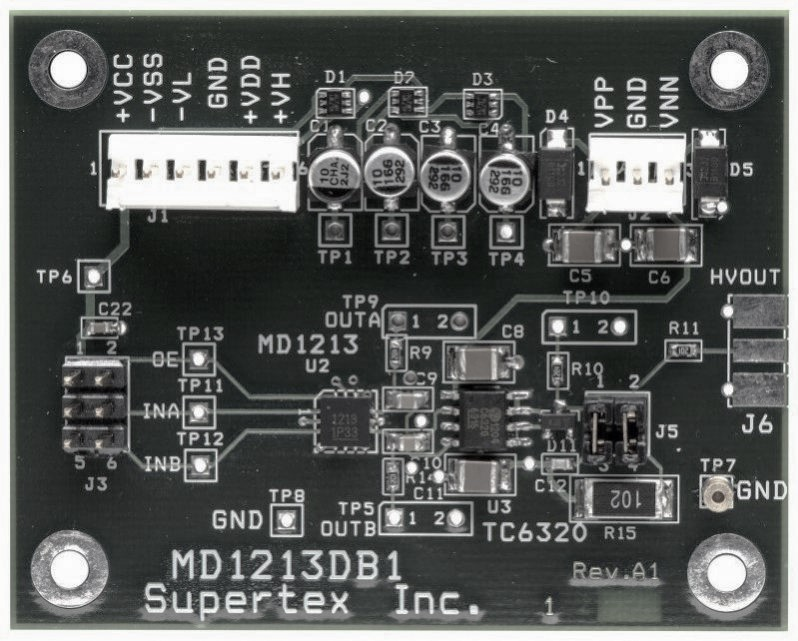
\includegraphics[width=.8\textwidth]{Figures/4_transmitter_pcb_pic.jpg}
	\caption{MD1213DB1 High Speed Pulser}
	\label{fig:4_transmitter_pcb_pic}
\end{figure}
\begin{figure}[htbp]
	\centering
	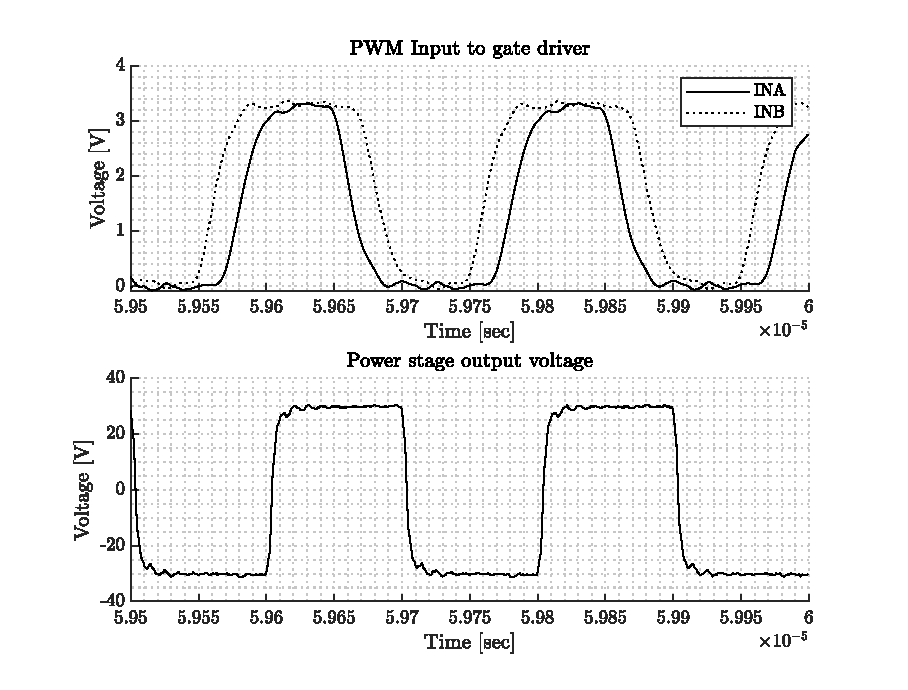
\includegraphics[width=.8\textwidth]{Figures/4_transmitter_pcb_out.eps}
	\caption[Measured input and output of power stage PCB]{Measured input and output of power stage PCB. (Above) Input to gate driver with dead-time (Below) Output of MOSFET half-bridge and the voltage across the load}
	\label{fig:4_transmitter_meas}
\end{figure}
Seen in \cref{fig:4_transmitter_meas} are actual measured inputs and outputs of the power stage. On the input, there are two complementary \qty{5}{\mega\hertz} signals with varying duty cycle to generate the desired dead-time. On the output, we see the rail-to-rail push-pull operation of the \gls{mosfet} half-bridge. The schematic of the transmitter can be found in the appendix in \cref{fig:appendix_md1213db1}.
\section{Transmit/Receive Switch}
\begin{figure}[htbp]
	\centering
	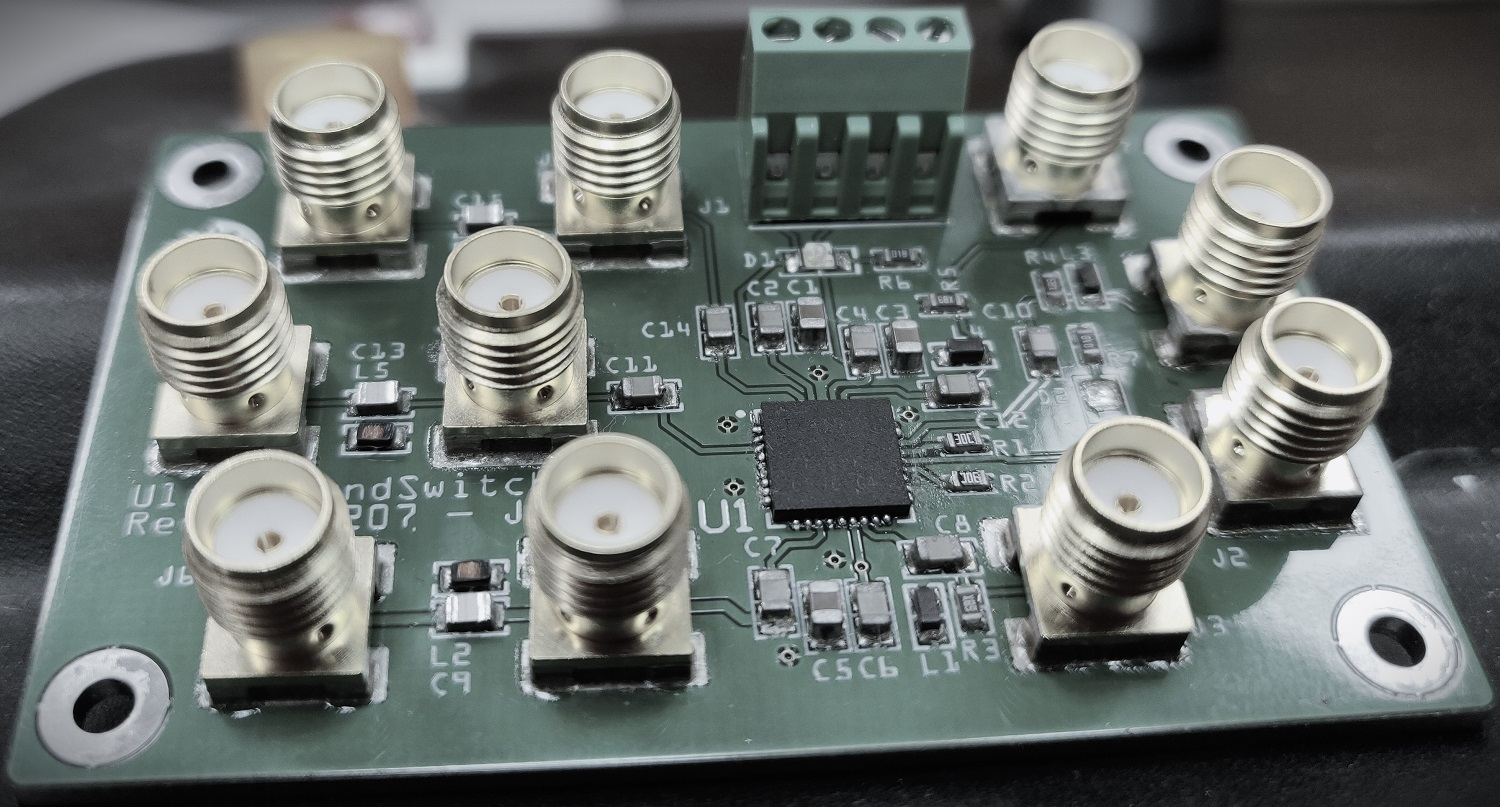
\includegraphics[width=.8\textwidth]{Figures/4_switch_pcb_pic.jpg}
	\caption[Transmit/Receive Switch after assembly]{Transmit/Receive Switch after assembly}
	\label{fig:4_txrx_pcb}
\end{figure}
The entire schematic of the transmit/receive switch can be found in the appendix in \cref{fig:appendix_ultrasoundswitch_a,fig:appendix_ultrasoundswitch_b}. As mentioned in the previous chapter, a PCB layout was made and a batch of 5 was ordered with an accompanying stencil for fast assembly.
\begin{figure}[htbp]
	\centering
	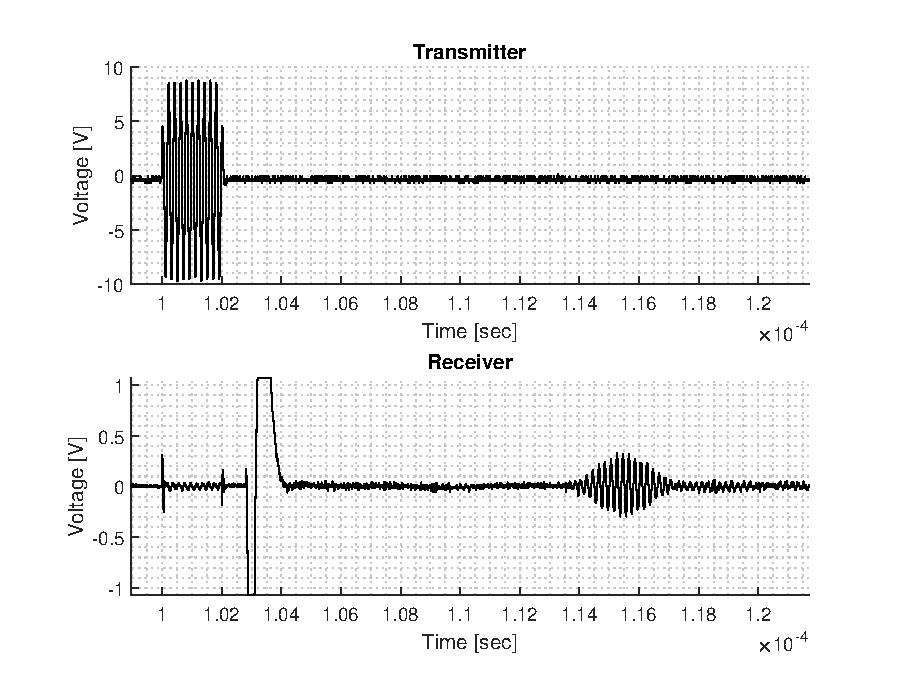
\includegraphics[width=.8\textwidth]{Figures/4_switch_pcb_meas.eps}
	\caption[Measured transmit and receive on Transmit/Receive Switch PCB]{Measured transmit and receive on Transmit/Receive Switch PCB (Above) Measured transmit voltage (Below) Received reflected signal off water tank}
	\label{fig:4_txrx_meas}
\end{figure}
\section{Preamplifier} \todo{Hvad er der galt med oscilloskopet?}
\begin{figure}[htbp]
	\centering
	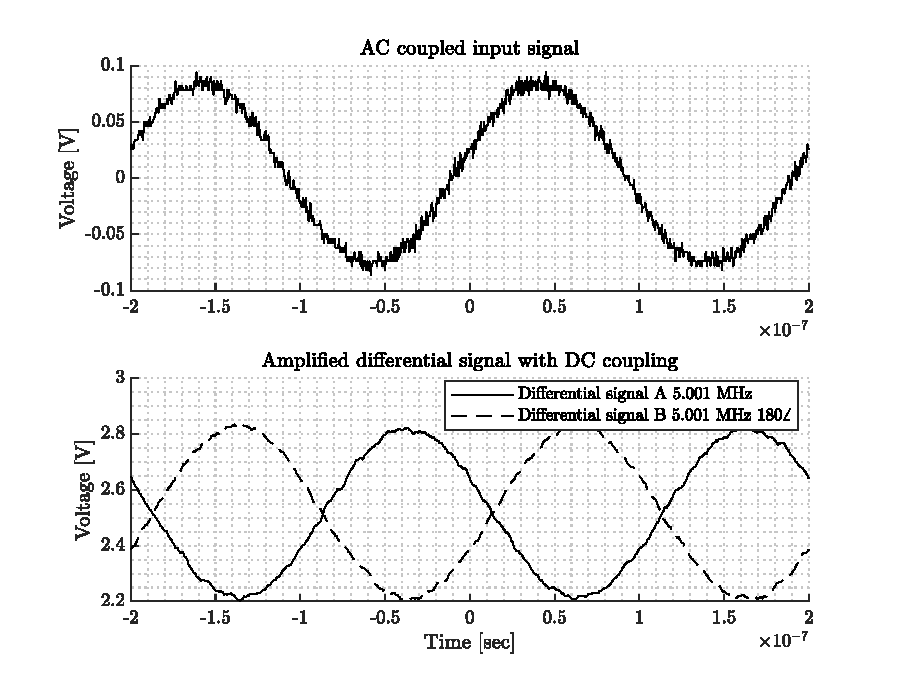
\includegraphics[width=.8\textwidth]{Figures/4_preamplifier_pcb.eps}
	\caption[Measured input of preamplifier PCB]{Measured input of preamplifier PCB, (Above) AC coupled input signal with amplitude \qty{1}{\volt} (Below Measured output of preamplifier PCB, Differential signal with DC coupling and $\times \qty{19}{\decibel}$ amplification)}
	\label{fig:4_preamp_in}
\end{figure}
%\begin{figure}[htbp]
%	\centering
%	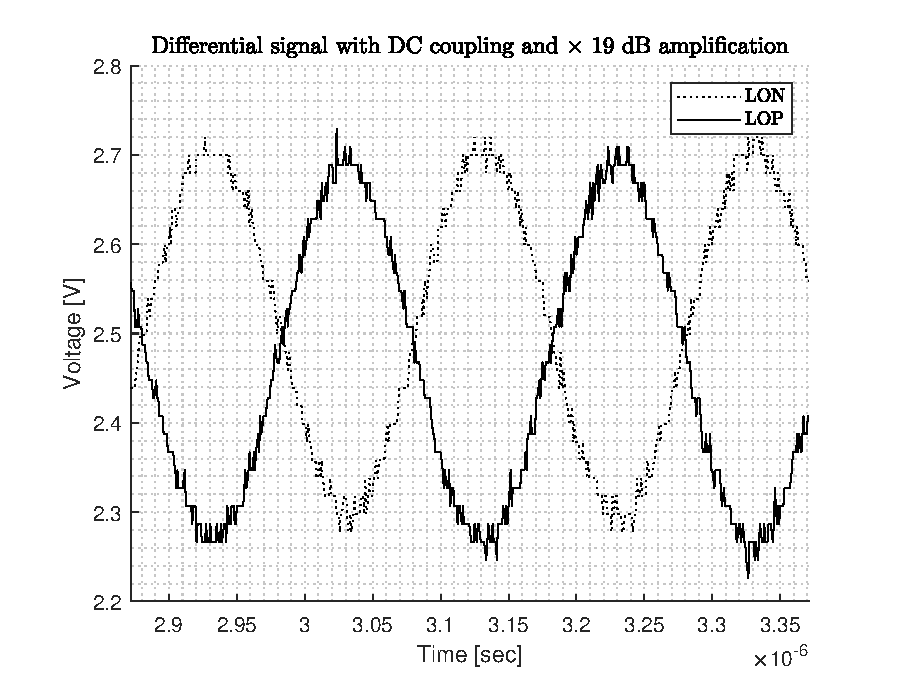
\includegraphics[width=.8\textwidth]{Figures/4_preamplifier_pcb_out.eps}
%	\caption[Measured output of preamplifier PCB]{Measured output of preamplifier PCB, Differential signal with DC coupling and $\times \qty{19}{\decibel}$ amplification}
%	\label{fig:4_preamp_out}
%\end{figure}
The entire schematic of the preamplifier can be found in the appendix in \cref{fig:appendix_ad8333}.
\section{Demodulator}
\begin{figure}[htbp]
	\centering
	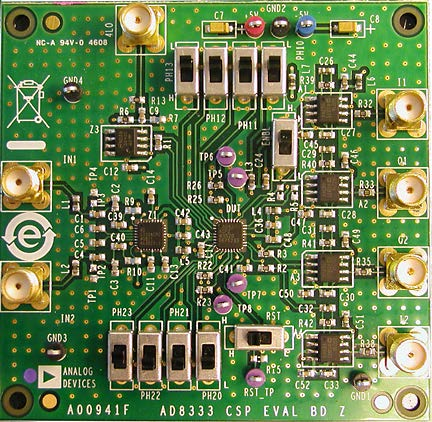
\includegraphics[width=.8\textwidth]{Figures/4_demod_pcb_pic.jpg}
	\caption{Demodulator PCB AD8333-EVALZ}
	\label{fig:4_demod_pcb_pic}
\end{figure}

\begin{figure}[htbp]
	\centering
	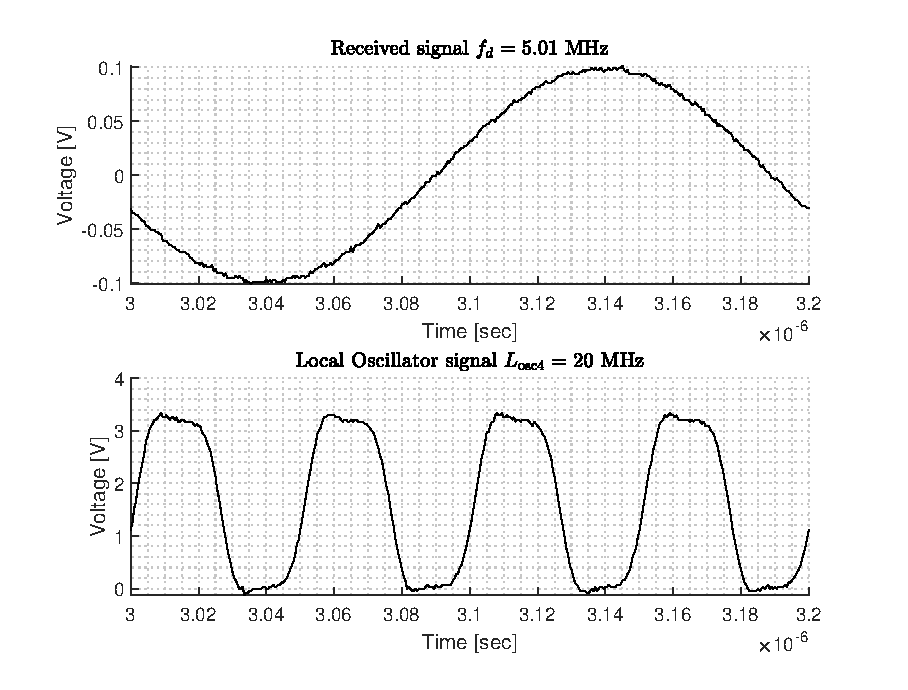
\includegraphics[width=.8\textwidth]{Figures/4_demod_pcb_in.eps}
	\caption[Measured input of demodulator PCB]{Measured input of demodulator PCB (Above) Input from received signal (Below) Input from local oscillator ($f_{0}\cdot4$)}
	\label{fig:4_demod_in}
\end{figure}
\begin{figure}[htbp]
	\centering
	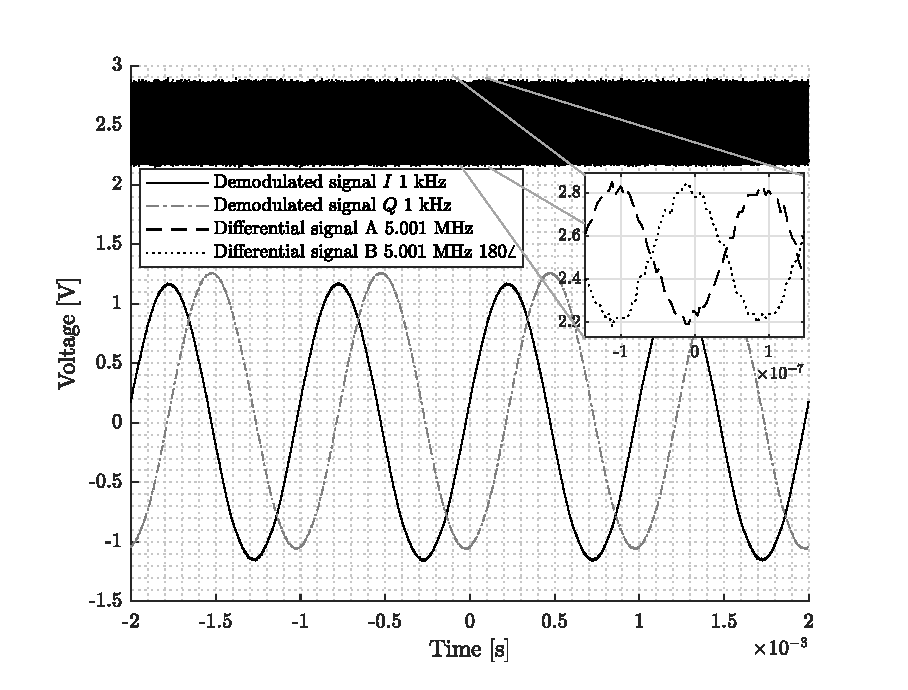
\includegraphics[width=.8\textwidth]{Figures/4_demod_pcb_out.eps}
	\caption[Measured output of demodulator PCB]{Measured output of demodulator PCB}
	\label{fig:4_demod_out}
\end{figure}
The entire schematic of the demodulator can be found in the appendix in \cref{fig:appendix_ad8333}.
\section{Sample and Hold}
\begin{figure}[htbp]
	\centering
	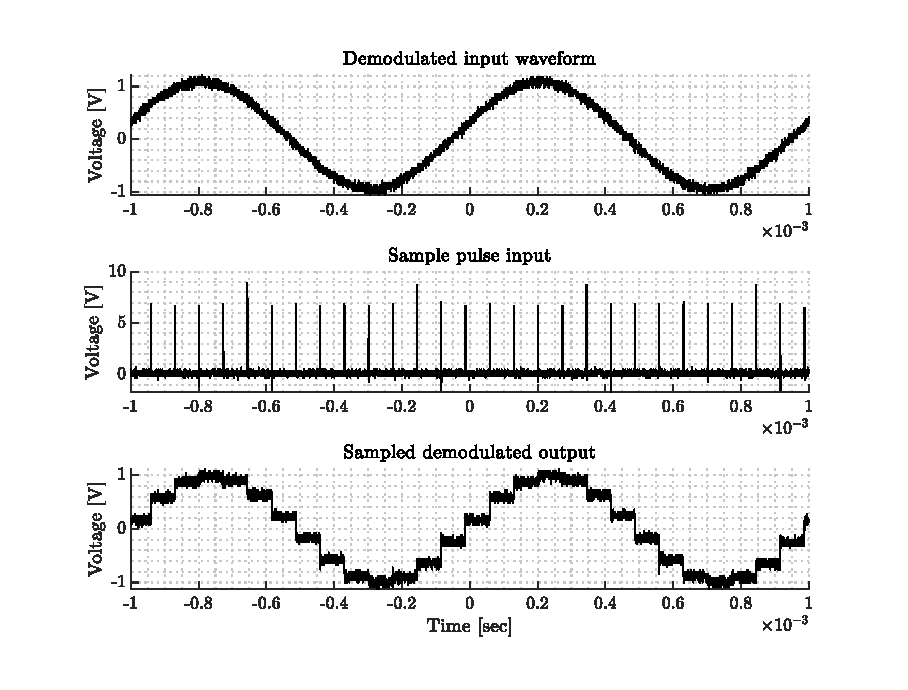
\includegraphics[width=.8\textwidth]{Figures/4_sampler_pcb.eps}
	\caption{Measured input and output of Sample and Hold amplifier}
	\label{fig:4_sample_hold_pcb}
\end{figure}

\section{Pulse-Repetition and Wall Filter}
\section{Digital Signal Processor}
%\begin{figure}[H]
%	\centering
%	\begin{circuitikz}[american voltages]
%		\draw
%		(0,0) to [short, *-] (6,0)
%		to [V, l_=$\mathrm{j}{\omega}_m \underline{\psi}^s_R$] (6,2)
%		to [R, l_=$R_R$] (6,4)
%		to [short, i_=$\underline{i}^s_R$] (5,4)
%		(0,0) to [open, v^>=$\underline{u}^s_s$] (0,4)
%		to [short, *- ,i=$\underline{i}^s_s$] (1,4)
%		to [R, l=$R_s$] (3,4)
%		to [L, l=$L_{\sigma}$] (5,4)
%		to [short, i_=$\underline{i}^s_M$] (5,3)
%		to [L, l_=$L_M$] (5,0);
%	\end{circuitikz}
%	\caption{The nodes short, V, R and L are presented here, but there a lot more}
%	\label{fig:circuitikz}
%\end{figure}
%
%\section{Listings (code)}
%
%\Cref{lst:helloworld} is a nicely formatted block of code. A listing will automatically continue on the next page if it encounters a page break. Many different programming languages can be highlighted. Check the \texttt{listings} package documentation for a list of supported programming languages.

%\begin{listing}[htbp]
%\begin{mintedc}
%#include <stdio.h>
%int main()
%{
%	printf("Hello, World!"); /*printf() outputs the quoted string*/
%	if (n == 0 || n == 1){
%		return n;
%	}
%	j = 0;
%	for (i = 0; i < n-1; i++){
%		if (arr[i] != arr[i+1]){
%			arr[j] = arr[i];
%			j++;
%		}
%	}
%	arr[j++] = arr[n-1];
%	return 0;
%}
%\end{mintedc}
%	\caption{Hello world in C}
%	\label{lst:helloworld}
%\end{listing}



